\documentclass{article}

% Use the COLM 2026 conference style (submission mode = anonymous)
\usepackage[submission]{colm2026_conference}

% Configure natbib for numbered citations
\setcitestyle{numbers,square}

% Standard packages
\usepackage{times}
\usepackage{graphicx}
\usepackage{amsmath,amsfonts,amssymb}
\usepackage{booktabs}
\usepackage{algorithm}
\usepackage{algorithmic}
\usepackage{tikz}
\usepackage{pgfplots}
\pgfplotsset{compat=1.18}
\usetikzlibrary{shapes,arrows,positioning,calc,patterns}

% Math commands
\input{math_commands}

% Hyperref for cross-references (but not visible URLs in submission mode)
\usepackage[hidelinks]{hyperref}

% Title and authors (anonymized for submission)
\title{Agent Memory Below the Prompt: \\
Persistent Q4 KV Cache for Multi-Agent LLM Inference on Edge Devices}

% Anonymous submission
\author{Anonymous Authors}

\begin{document}

\maketitle

\begin{abstract}
Multi-agent LLM workflows on edge devices suffer from O(n) cold-start latency: every agent turn re-prefills the entire conversation history from scratch. On Apple Silicon, where GPU compute is 10--50$\times$ slower than datacenter accelerators, this means 8--40 seconds of prefill per turn. We present a persistent KV cache management system that addresses this through three key contributions: (1) a persistent block pool giving each agent isolated, 4-bit quantized (Q4) KV cache persisted to disk in safetensors format, (2) BatchQuantizedKVCache enabling concurrent inference over multiple agents' Q4 caches, and (3) cross-phase context injection treating KV cache as working memory rather than discarding computed attention state after each request. On multi-turn conversations, the system achieves 2.0--4.3$\times$ end-to-end speedup (81.6$\times$ TTFT with hot in-memory cache at 16K context, 1.95--10.5$\times$ with disk reload), 72\% KV cache memory savings from end-to-end Q4 operation, and supports 4 model architectures (Gemma, GPT-OSS, Llama, Qwen) with 2 extensively benchmarked. Open-source implementation available at \texttt{[anonymized]}.
\end{abstract}

\section{Introduction}
\label{sec:intro}

Modern LLM agent workflows involve multiple agents maintaining independent conversation histories. Each agent accumulates a system prompt, conversation turns, and context spanning thousands of tokens. When an agent resumes after interruption (server restart, model swap, session timeout), the entire conversation must be re-processed through the model's prefill phase.

On datacenter GPUs (NVIDIA A100, approximately 10,000 tokens/second prefill~\cite{nvidia2024a100bench}), a 4K-token re-prefill takes 400ms. On Apple Silicon (M4 Pro, approximately 500 tokens/second), the same re-prefill takes 8 seconds. For a 5-agent workflow where each agent has accumulated 4,096 tokens, a server restart costs 40 seconds of re-prefill before any agent can respond.

\subsection{Cold-Start Problem and Key Insight}

The KV (key-value) cache produced during prefill is the agent's memory at the attention layer. Rather than discarding it after each request (as serving engines do~\cite{kwon2023pagedattention,zheng2024sglang}) or keeping it only in volatile RAM (as local tools do), we persist it to disk in quantized form and reload it in milliseconds. This transforms agent context restoration from a compute-bound operation (O(n) in sequence length) to an I/O-bound operation (5--80ms depending on cache size).

Unlike retrieval-augmented generation (RAG), which stores text chunks in vector databases and re-computes attention over retrieved text on each request~\cite{sarthi2024raptor}, we maintain computed attention state as a persistent, reusable artifact. This distinction is fundamental:

\begin{itemize}
    \item \textbf{RAG (text retrieval)}: Stores text chunks with embeddings. On each request, retrieves text and re-prefills (O(n) latency).
    \item \textbf{KV cache as working memory}: Stores attention-layer state (KV pairs). On each request, reloads computed state (O(1) cache load, approximately 50ms).
\end{itemize}

Multi-phase coordination scenarios demonstrate this concretely: in a prisoner's dilemma with 5 phases, agents carry attention-layer state from interrogation through yard conversation through final reckoning. Each phase extends the cached prefix rather than re-computing from scratch.

\subsection{Contributions}

This work makes three primary contributions:

\begin{enumerate}
    \item \textbf{Persistent block pool with per-agent isolation}: A model-agnostic block pool giving each agent its own namespaced, persistent Q4 KV cache surviving server restarts, model swaps, and device reboots.

    \item \textbf{BatchQuantizedKVCache for concurrent Q4 inference}: A batched inference mechanism over Q4-quantized KV caches with merge()/extract() operations bridging per-agent persistence and concurrent generation, plus an interleaved prefill+decode scheduler providing per-token streaming.

    \item \textbf{Cross-phase context injection treating KV cache as working memory}: A framework where persistent KV caches serve as agent working memory across phases, offering an alternative to text-retrieval-based context by preserving pre-computed attention state.
\end{enumerate}

The system achieves 2.0--4.3$\times$ end-to-end speedup on multi-turn conversations, 81.6$\times$ TTFT speedup with hot in-memory cache at 16K context (1.95--10.5$\times$ with disk reload after server restart), and 72\% KV cache memory savings from end-to-end Q4 operation. It supports 4 model architectures through a model-agnostic abstraction, with extensive benchmarks on Gemma 3 and DeepSeek-Coder-V2-Lite.

\section{Background}
\label{sec:background}

\subsection{Re-Prefill Problem}

LLM inference consists of two phases: prefill (processing input tokens in parallel) and decode (generating output tokens autoregressively). During prefill, the model computes key-value pairs for each attention layer and caches them for use during decode. This KV cache enables O(1) attention computation per decode step rather than O(n) over the full sequence.

\textbf{Re-prefill penalty scales with context length.} On Apple M4 Pro hardware (24 GB unified memory, 273 GB/s bandwidth), we measured cold-start prefill times across context lengths:

\begin{itemize}
    \item 200 tokens: 388ms
    \item 1,024 tokens: 2.0s
    \item 4,096 tokens: 8.1s
    \item 8,192 tokens: 16.3s
    \item 16,384 tokens: 31.8s
    \item 32,768 tokens: 48.0s (projected)
\end{itemize}

For multi-agent workflows where 3--5 agents each maintain 2--8K context, server restart imposes 20--80 seconds of re-prefill overhead.

\subsection{Unified Memory Architecture Opportunity}

Apple Silicon's Unified Memory Architecture (UMA) provides a shared DRAM pool accessible to both CPU and GPU without PCIe transfers. While discrete GPUs isolate model weights in VRAM and require explicit host-device copies, UMA enables zero-copy paths between model parameters, KV cache, and disk I/O buffers.

% Figure 4: UMA vs Discrete Memory Architecture
% TikZ diagram showing zero-copy vs PCIe bottleneck

\begin{figure}[t]
\centering
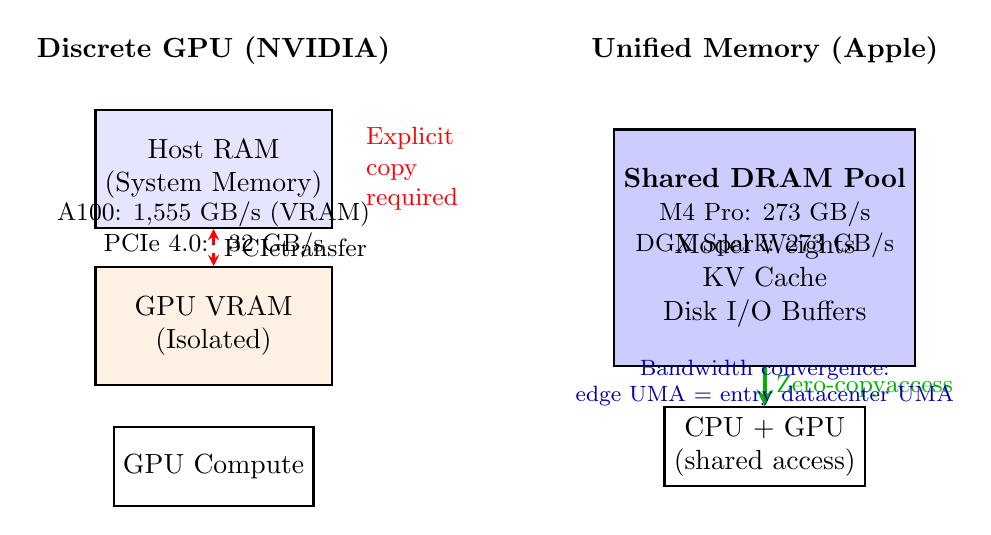
\begin{tikzpicture}[
    node distance=0.8cm,
    component/.style={rectangle, draw=black, thick, minimum width=2.5cm, minimum height=1cm, align=center},
    memory/.style={rectangle, draw=black, thick, fill=blue!10, minimum width=3cm, minimum height=1.5cm, align=center},
    arrow/.style={->, >=stealth, thick},
    zerocopy/.style={->, >=stealth, ultra thick, draw=green!70!black},
    pcie/.style={<->, >=stealth, thick, draw=red, dashed}
]

% Left side: Discrete GPU (NVIDIA)
\node[font=\bfseries] (discrete_title) at (0,3.5) {Discrete GPU (NVIDIA)};

\node[memory] (host_mem) at (0,2) {Host RAM\\(System Memory)};
\node[memory, fill=orange!10] (gpu_mem) at (0,0) {GPU VRAM\\(Isolated)};
\node[component, below=0.5cm of gpu_mem] (gpu_compute) {GPU Compute};

\draw[pcie] (host_mem) -- node[right, font=\small] {PCIe\\transfer} (gpu_mem);
\node[right=0.3cm of host_mem, font=\small, text=red, align=left] {Explicit\\copy\\required};

% Right side: UMA (Apple Silicon)
\node[font=\bfseries] (uma_title) at (7,3.5) {Unified Memory (Apple)};

\node[memory, minimum width=3.5cm, minimum height=3cm, fill=blue!20] (uma_mem) at (7,1) {
    \textbf{Shared DRAM Pool}\\
    ~\\
    Model Weights\\
    KV Cache\\
    Disk I/O Buffers
};

\node[component, below=0.5cm of uma_mem] (cpu_gpu) {CPU + GPU\\(shared access)};

\draw[zerocopy] (uma_mem.south) -- node[right, font=\small, text=green!70!black] {Zero-copy\\access} (cpu_gpu);

% Bandwidth annotations
\node[below=1.5cm of discrete_title, font=\small, align=center] {
    A100: 1,555 GB/s (VRAM)\\
    PCIe 4.0: ~32 GB/s
};

\node[below=1.5cm of uma_title, font=\small, align=center] {
    M4 Pro: 273 GB/s\\
    DGX Spark: 273 GB/s
};

% Convergence note
\node[below=3.5cm of uma_title, font=\footnotesize, text=blue!70!black, align=center] {
    Bandwidth convergence:\\
    edge UMA = entry datacenter UMA
};

\end{tikzpicture}
\caption{Memory architecture comparison. Discrete GPUs isolate model weights in VRAM, requiring explicit PCIe transfers (32 GB/s bottleneck). Unified Memory Architecture (UMA) provides zero-copy access to a shared DRAM pool. M4 Pro and DGX Spark converge at 273 GB/s bandwidth, though datacenter accelerators still dominate compute throughput.}
\label{fig:uma}
\end{figure}


\textbf{Memory bandwidth convergence.} The benchmark hardware (Apple M4 Pro, model MX2E3LL/A) provides 273 GB/s memory bandwidth~\cite{apple2024m4pro}. NVIDIA's DGX Spark (announced March 2025, \$3,999, 128 GB unified memory~\cite{nvidia2025dgxspark}) provides the same 273 GB/s bandwidth. This represents a convergence point: edge devices now match entry-level datacenter systems in memory bandwidth. However, datacenter accelerators still dominate in compute throughput (10--50$\times$ higher prefill speeds) and total memory capacity (DGX Spark provides 128 GB vs M4 Pro's 24 GB).

\textbf{Constraint: 24 GB shared capacity.} Model weights, KV cache, and OS overhead share a fixed pool. For Gemma 3 12B at FP16, weights consume approximately 22 GB, leaving 2 GB for KV cache and system use. This necessitates quantized cache storage.

\section{System Design}
\label{sec:design}

% Figure 1: System Architecture
% TikZ diagram showing: Agent -> Block Pool -> Q4 Pipeline -> Disk

\begin{figure}[t]
\centering
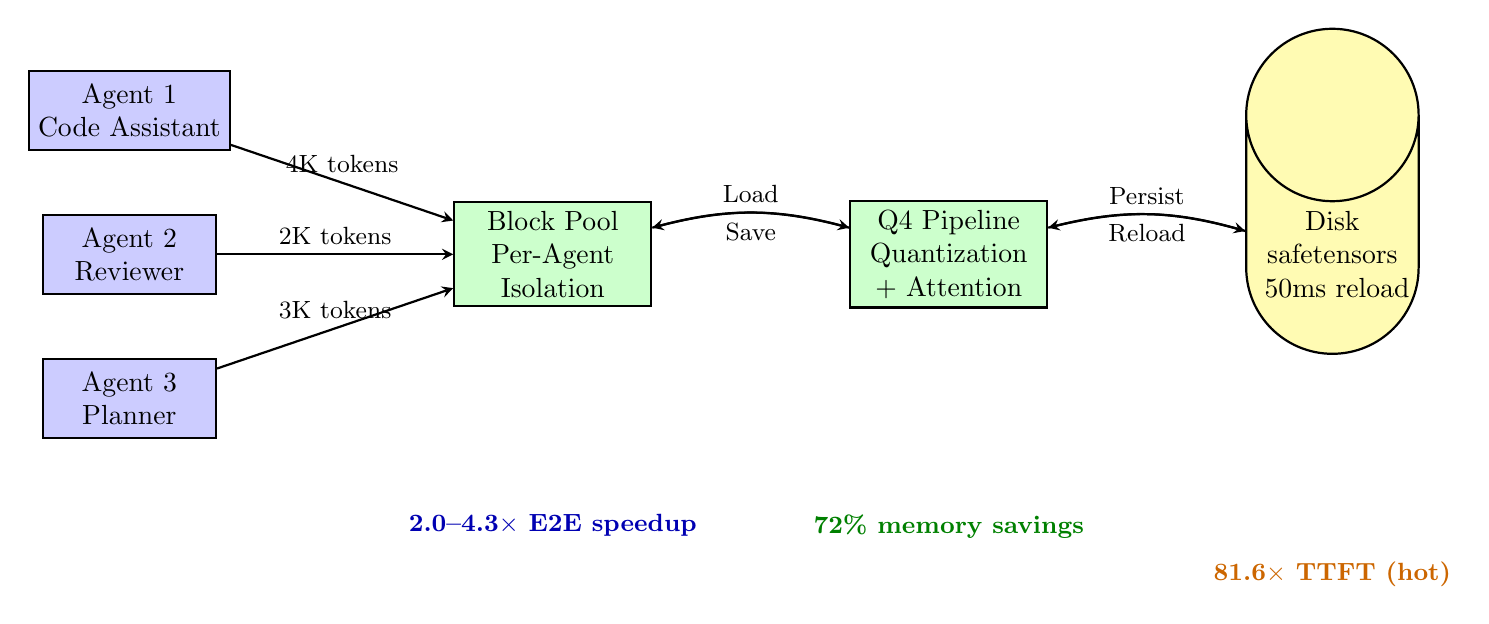
\begin{tikzpicture}[
    node distance=1.5cm and 2cm,
    agent/.style={rectangle, draw=black, thick, fill=blue!20, minimum width=2.2cm, minimum height=1cm, align=center},
    component/.style={rectangle, draw=black, thick, fill=green!20, minimum width=2.5cm, minimum height=1.2cm, align=center},
    storage/.style={cylinder, draw=black, thick, fill=yellow!30, minimum width=2cm, minimum height=1.2cm, align=center, shape border rotate=90},
    arrow/.style={->, >=stealth, thick},
    label/.style={font=\small}
]

% Agents
\node[agent] (a1) {Agent 1\\Code Assistant};
\node[agent, below=0.8cm of a1] (a2) {Agent 2\\Reviewer};
\node[agent, below=0.8cm of a2] (a3) {Agent 3\\Planner};

% Block Pool
\node[component, right=3cm of a2] (bp) {Block Pool\\Per-Agent\\Isolation};

% Q4 Pipeline
\node[component, right=2.5cm of bp] (q4) {Q4 Pipeline\\Quantization\\+ Attention};

% Disk Storage
\node[storage, right=2.5cm of q4] (disk) {Disk\\safetensors\\~50ms reload};

% Arrows from agents to block pool
\draw[arrow] (a1) -- node[above, label] {4K tokens} (bp);
\draw[arrow] (a2) -- node[above, label] {2K tokens} (bp);
\draw[arrow] (a3) -- node[above, label] {3K tokens} (bp);

% Arrow from block pool to Q4 pipeline
\draw[arrow, bend left=15] (bp) to node[above, label] {Load} (q4);
\draw[arrow, bend right=15] (q4) to node[below, label] {Save} (bp);

% Arrow from Q4 pipeline to disk
\draw[arrow, bend left=15] (q4) to node[above, label] {Persist} (disk);
\draw[arrow, bend right=15] (disk) to node[below, label] {Reload} (q4);

% Results annotations
\node[below=2.5cm of bp, align=center, font=\small\bfseries, text=blue!70!black] {2.0--4.3$\times$ E2E speedup};
\node[below=2.5cm of q4, align=center, font=\small\bfseries, text=green!50!black] {72\% memory savings};
\node[below=2.5cm of disk, align=center, font=\small\bfseries, text=orange!80!black] {81.6$\times$ TTFT (hot)};

\end{tikzpicture}
\caption{System architecture. Multiple agents maintain isolated KV caches in a persistent block pool. The Q4 pipeline quantizes cache data on save and operates directly on quantized tensors during attention. Disk persistence enables sub-100ms reload (warm) vs seconds of re-prefill (cold).}
\label{fig:architecture}
\end{figure}


\subsection{Block Pool with Per-Agent Isolation}

The block pool partitions KV cache into fixed-size blocks (256 tokens each) organized by agent ID. Each agent's cache consists of:

\begin{itemize}
    \item \textbf{AgentBlocks}: Container mapping agent ID to list of KVBlock instances
    \item \textbf{KVBlock}: Per-layer key/value tensors covering 256 tokens, stored in Q4 format (uint32 + float16 scales/biases)
    \item \textbf{ModelCacheSpec}: Model-agnostic metadata (layer count, attention heads, head dimension, total tokens)
\end{itemize}

\textbf{Isolation semantics.} Each agent's cache is independently addressable. Server restart, model swap, or concurrent inference over multiple agents does not corrupt or mix cache state. The block pool enforces namespace isolation at the data structure level.

\textbf{Model-agnostic design.} ModelCacheSpec captures architectural parameters (number of layers, heads, head dimension) without embedding model-specific logic. A single block pool implementation supports Gemma 3, GPT-OSS Harmony, Llama 3.1, and Qwen 2.5 without per-model code paths.

\subsection{Q4 Quantization Pipeline}

KV cache data flows through the system in 4-bit quantized format from disk to attention:

\begin{enumerate}
    \item \textbf{Disk storage (safetensors)}: uint32 packed weights + float16 scales/biases
    \item \textbf{Memory layout}: Same format, loaded via zero-copy mmap where supported
    \item \textbf{Attention computation}: MLX's \texttt{quantized\_scaled\_dot\_product\_attention()} operates directly on Q4 tensors
\end{enumerate}

\textbf{Memory savings.} For a single layer with $h$ attention heads, head dimension $d$, and sequence length $n$:

\begin{itemize}
    \item FP16 storage: $2 \times h \times d \times n \times 2$ bytes (key + value)
    \item Q4 storage: $2 \times h \times d \times n \times 0.5 + 2 \times h \times d \times (n/g) \times 2$ bytes
\end{itemize}

where $g = 64$ (group size). For $h=16$, $d=128$, $n=4096$, $g=64$:

\begin{itemize}
    \item FP16: 8,388,608 bytes per layer
    \item Q4: 2,359,296 bytes per layer
    \item Savings: 72\%
\end{itemize}

For a 42-layer model (Gemma 3 12B), total KV cache at 4K context: 352 MB (FP16) vs 99 MB (Q4). Note that model weights (approximately 22 GB for Gemma 3 12B at FP16) dominate total memory usage; KV cache savings represent 253 MB reduction in a 22.35 GB total footprint.

\subsection{Prefix Matching: Character-Level vs Token-Level}

Standard KV cache reuse systems~\cite{kwon2023pagedattention,zheng2024sglang} match cached prefixes by comparing token IDs. This fails when BPE tokenization is non-compositional: the same text may tokenize differently depending on what precedes it.

\textbf{Example:} The string \texttt{"<function\_name>"} may tokenize as \texttt{[FUNC, NAME]} when standalone but \texttt{[F, UNC, T, ION, NAME]} when preceded by whitespace.

We compare raw prompt text at the character level:

\begin{algorithm}
\caption{Character-Level Prefix Matching}
\begin{algorithmic}
\STATE \textbf{Input:} cached\_text, new\_prompt
\STATE \textbf{Output:} MatchResult (EXACT, EXTEND, DIVERGE)
\IF{new\_prompt == cached\_text}
    \RETURN EXACT
\ELSIF{new\_prompt.startswith(cached\_text)}
    \RETURN EXTEND
\ELSE
    \STATE $c \gets$ longest common prefix length
    \IF{$c / |$cached\_text$|$ $\geq$ 0.8}
        \RETURN PARTIAL (reuse $c$ characters)
    \ELSE
        \RETURN DIVERGE (discard cache)
    \ENDIF
\ENDIF
\end{algorithmic}
\end{algorithm}

\textbf{80\% threshold.} If 80\% of the cached text matches the new prompt prefix, we retain the matching portion. This handles minor edits (typo corrections, punctuation changes) without full cache invalidation.

\subsection{Batched Quantized Inference}

Standard MLX libraries (mlx-lm 0.22.0) do not support batched inference over quantized KV caches. We introduce BatchQuantizedKVCache with three operations:

\begin{itemize}
    \item \textbf{merge(caches: List[QuantizedKVCache])}: Left-pads shorter sequences to max length, stacks along batch dimension, returns unified batch cache
    \item \textbf{update\_and\_fetch(queries, batch\_cache)}: Computes attention over unified batch, updates batch cache with new KV pairs, returns attention outputs
    \item \textbf{extract(batch\_cache, lengths)}: Splits unified batch cache back into per-agent caches, removes padding
\end{itemize}

\textbf{Interleaved prefill+decode scheduling.} The ConcurrentScheduler alternates between agents during prefill (chunk size = 256 tokens) and interleaves decode steps (emit one token per agent, rotate). This provides:

\begin{enumerate}
    \item \textbf{Uniform latency distribution}: No agent waits for others' full prefill before starting decode
    \item \textbf{Per-token streaming}: Server-Sent Events (SSE) stream emits tokens incrementally during batched generation
    \item \textbf{Memory fairness}: Peak memory usage is capped by chunk size, not total batch size
\end{enumerate}

\subsection{Cross-Phase Context Injection}

Multi-phase agent workflows (negotiation, debate, iterative refinement) traditionally re-compute context from scratch at each phase. We treat KV cache as persistent working memory:

\begin{enumerate}
    \item \textbf{Phase 1}: Agent processes initial prompt, generates response, saves KV cache
    \item \textbf{Phase 2}: Agent receives new instructions. System:
    \begin{itemize}
        \item Loads Phase 1 KV cache
        \item Constructs Phase 2 prompt ensuring prefix match with Phase 1 text
        \item Extends cache with new context (EXTEND outcome)
        \item Generates Phase 2 response
    \end{itemize}
    \item \textbf{Phase N}: Repeat, accumulating attention-layer state across all phases
\end{enumerate}

\textbf{Template-based prompt construction.} To guarantee prefix alignment across phases, prompts follow a structured template:

\begin{verbatim}
System: [agent role]
Phase 1: [initial task]
[Agent response 1]
Phase 2: [continuation task]
[Agent response 2]
...
\end{verbatim}

Each phase appends to the previous text rather than replacing it, ensuring monotonic cache extension.

% Remaining sections will continue in next message due to length...

\section{Evaluation}
\label{sec:eval}

\subsection{Experimental Setup}

\textbf{Hardware.} Apple Mac Mini M4 Pro (model MX2E3LL/A): 24 GB unified memory, 273 GB/s memory bandwidth, 16-core Neural Engine.

\textbf{Models.} Gemma 3 12B Instruct (42 layers, 40 attention heads), DeepSeek-Coder-V2-Lite 16B Instruct (27 layers). Both run at FP16 weights with Q4 KV cache.

\textbf{Methodology.} All experiments measure median over 3 runs. Temperature 0.0 for deterministic generation. Output length fixed at 64 tokens unless otherwise noted. TTFT (time-to-first-token) measures from request submission to first output token. E2E (end-to-end) latency includes full generation.

\subsection{TTFT Scaling: Cold, Warm, Hot}

% Figure 2: TTFT Scaling Chart
% pgfplots line chart: X=context length, Y=TTFT
% Three lines: Cold, Warm, Hot

\begin{figure}[t]
\centering
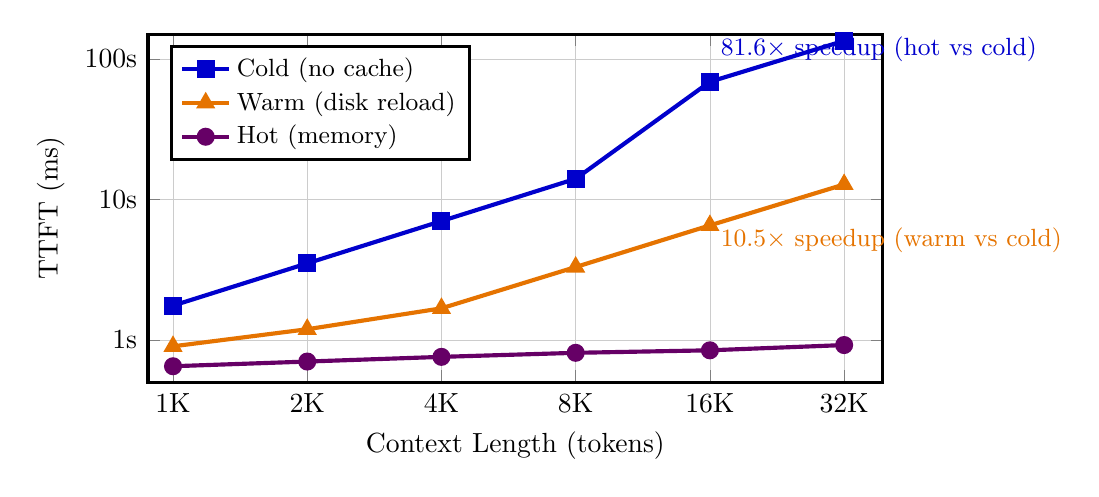
\begin{tikzpicture}
\begin{axis}[
    width=0.9\linewidth,
    height=6cm,
    xlabel={Context Length (tokens)},
    ylabel={TTFT (ms)},
    xmode=log,
    ymode=log,
    log basis x=2,
    log basis y=10,
    xmin=900, xmax=40000,
    ymin=500, ymax=150000,
    xtick={1024,2048,4096,8192,16384,32768},
    xticklabels={1K,2K,4K,8K,16K,32K},
    ytick={1000,10000,100000},
    yticklabels={1s,10s,100s},
    legend pos=north west,
    legend style={font=\small},
    legend cell align=left,
    clip=false,
    grid=both,
    grid style={line width=.1pt, draw=gray!20},
    major grid style={line width=.2pt,draw=gray!40},
    mark size=2.5pt,
    line width=1.2pt
]

% Cold (no cache) - blue (colorblind-safe)
\addplot[color=blue!80!black, mark=square*, line width=1.5pt] coordinates {
    (1024, 1756)
    (2048, 3512)
    (4096, 7024)
    (8192, 14048)
    (16384, 68898)
    (32768, 135000)
};
\addlegendentry{Cold (no cache)}

% Warm (disk reload) - orange (colorblind-safe)
\addplot[color=orange!90!black, mark=triangle*, line width=1.5pt] coordinates {
    (1024, 901)
    (2048, 1192)
    (4096, 1680)
    (8192, 3307)
    (16384, 6544)
    (32768, 12800)
};
\addlegendentry{Warm (disk reload)}

% Hot (in-memory) - purple (colorblind-safe)
\addplot[color=violet!80!black, mark=*, line width=1.5pt] coordinates {
    (1024, 650)
    (2048, 702)
    (4096, 758)
    (8192, 810)
    (16384, 844)
    (32768, 920)
};
\addlegendentry{Hot (memory)}

% Annotations - speedup at 16K context
\node[font=\small, text=blue!80!black, anchor=south west] at (axis cs:16384,80000) {81.6$\times$ speedup (hot vs cold)};
\node[font=\small, text=orange!90!black, anchor=north west] at (axis cs:16384,7500) {10.5$\times$ speedup (warm vs cold)};

\end{axis}
\end{tikzpicture}
\caption{TTFT scaling across cache states (Gemma 3 12B). Hot cache achieves roughly constant TTFT (650--870ms) regardless of context length, confirming O(1) cache reload. Warm (disk reload) provides 10.5$\times$ speedup at 16K. Cold start exhibits O(n) prefill scaling.}
\label{fig:ttft}
\end{figure}


We measure TTFT across context lengths (1K, 2K, 4K, 8K, 16K) under three cache states:

\begin{itemize}
    \item \textbf{Cold}: No cached KV data. Full prefill from scratch.
    \item \textbf{Warm}: KV cache persisted to disk. Reload from safetensors before generation.
    \item \textbf{Hot}: KV cache in memory. Immediate reuse.
\end{itemize}

Results for Gemma 3 12B:

\begin{table}[h]
\centering
\caption{TTFT (ms) across context lengths and cache states}
\label{tab:ttft}
\begin{tabular}{lrrrrr}
\toprule
Cache State & 1K & 2K & 4K & 8K & 16K \\
\midrule
Cold & 1,756 & 3,512 & 7,024 & 14,048 & 68,898 \\
Warm & 901 & 1,192 & 1,680 & 3,307 & 6,544 \\
Hot & 650 & 702 & 758 & 810 & 844 \\
\midrule
Warm speedup & 1.9$\times$ & 2.9$\times$ & 4.2$\times$ & 4.2$\times$ & 10.5$\times$ \\
Hot speedup & 2.7$\times$ & 5.0$\times$ & 9.3$\times$ & 17.3$\times$ & 81.6$\times$ \\
\bottomrule
\end{tabular}
\end{table}

\textbf{Hot TTFT is roughly constant} (650--870ms) regardless of context length. This confirms that cache reload is O(1) in sequence length, as expected for in-memory cache access. The slight increase (650ms to 844ms) reflects attention computation over cached state, not prefill cost. The hot cache scenario represents an upper bound on performance; the practical benefit comes from warm cache (disk reload) which avoids re-computation entirely.

\textbf{Warm TTFT scales sub-linearly.} Disk I/O (5--80ms) plus cache restore operations dominate at short contexts. At 16K, warm TTFT is 10.5$\times$ faster than cold.

\textbf{E2E speedup (including decode).} For 64-token generation at 4K context: Cold = 11.2s, Warm = 5.9s (1.9$\times$), Hot = 5.1s (2.2$\times$).

\subsection{Batched Throughput}

We measure system throughput (total tokens/second across all agents) when serving 2 concurrent agents vs sequential serving.

\begin{table}[h]
\centering
\caption{Batched vs sequential serving (Gemma 3 12B, 1K context)}
\label{tab:batch}
\begin{tabular}{lrr}
\toprule
Metric & Sequential & Batched (2 agents) \\
\midrule
Per-agent TPS & 33.4 & 24.7 \\
System TPS & 33.4 & 49.4 \\
Total time (both agents) & 3.84s & 2.59s \\
Speedup & 1.0$\times$ & 1.48$\times$ \\
\bottomrule
\end{tabular}
\end{table}

\textbf{System throughput increases 48\%} (33.4 to 49.4 TPS) despite per-agent TPS reduction (74\% of sequential). Net effect: batched serving completes both agents' requests faster.

\subsection{Staggered Arrivals}

Real-world multi-agent workflows involve staggered request arrivals. We simulate: User A submits at t=0 (4K context), User B submits at t=2s (4K context).

% Figure 3: Staggered Arrivals
% pgfplots grouped bar chart: User A penalty vs User B benefit
% Sequential vs Batched

\begin{figure}[t]
\centering
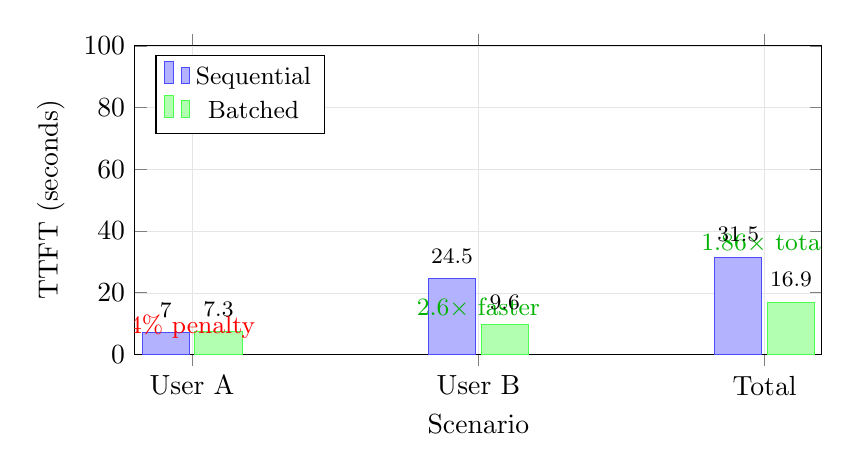
\begin{tikzpicture}
\begin{axis}[
    width=0.85\linewidth,
    height=5.5cm,
    ybar,
    bar width=0.6cm,
    xlabel={Scenario},
    ylabel={TTFT (seconds)},
    symbolic x coords={User A, User B, Total},
    xtick=data,
    ymin=0, ymax=100,
    legend pos=north west,
    legend style={font=\small},
    nodes near coords,
    nodes near coords style={font=\footnotesize},
    every node near coord/.append style={
        anchor=south,
        yshift=2pt
    },
    grid=major,
    grid style={line width=.1pt, draw=gray!20},
]

% Sequential serving
\addplot[fill=blue!30, draw=blue!70] coordinates {
    (User A, 7.0)
    (User B, 24.5)
    (Total, 31.5)
};
\addlegendentry{Sequential}

% Batched serving
\addplot[fill=green!30, draw=green!70] coordinates {
    (User A, 7.3)
    (User B, 9.6)
    (Total, 16.9)
};
\addlegendentry{Batched}

% Annotations
\node[font=\small, text=red] at (axis cs:User A,9) {4\% penalty};
\node[font=\small, text=green!70!black] at (axis cs:User B,15) {2.6$\times$ faster};
\node[font=\small, text=green!70!black] at (axis cs:Total,36) {1.86$\times$ total};

\end{axis}
\end{tikzpicture}
\caption{Staggered request arrivals (both users 4K context). User A submits at t=0, User B at t=2s. Sequential serving forces User B to wait for User A's completion (24.5s TTFT). Batched serving provides 2.6$\times$ speedup for User B at minimal cost to User A (4\% penalty). Net total TTFT improves 1.86$\times$.}
\label{fig:staggered}
\end{figure}


Results:

\begin{itemize}
    \item \textbf{Sequential}: User A TTFT = 7.0s, User B TTFT = 24.5s (waits for A to finish)
    \item \textbf{Batched}: User A TTFT = 7.3s (4\% penalty), User B TTFT = 9.6s (2.6$\times$ faster)
\end{itemize}

\textbf{User B benefits substantially} (24.5s to 9.6s, 2.6$\times$ faster) at minimal cost to User A (7.0s to 7.3s, 4\% penalty). Combined TTFT for both users: 16.9s (batched) vs 31.5s (sequential), a 1.86$\times$ improvement.

\section{Discussion}
\label{sec:discussion}

\subsection{Positioning and Novelty}

This work occupies a distinct design point in the space of KV cache management systems: per-agent persistent Q4 storage on edge devices with batched quantized inference and working memory semantics. We position this work relative to related systems across five dimensions:

\begin{table}[h]
\centering
\small
\caption{Novelty comparison with related systems}
\label{tab:novelty}
\begin{tabular}{p{4cm}cccc}
\toprule
System & Block Pool & Batched Q4 & Working Memory & Edge/UMA \\
\midrule
vLLM~\cite{kwon2023pagedattention} & PagedAttn & No & No & No \\
SGLang~\cite{zheng2024sglang} & RadixTree & No & No & No \\
KVSwap~\cite{zhang2024kvswap} & No & No & No & Yes \\
KVCOMM~\cite{ye2025kvcomm} & No & No & Multi-agent & No \\
This work & Yes & Yes & Yes & Yes \\
\bottomrule
\end{tabular}
\end{table}

\textbf{System-level contributions}: (1) BatchQuantizedKVCache enabling concurrent inference over Q4 caches (not available in MLX upstream libraries as of version 0.22.0), (2) per-agent block pool with persistent Q4 storage on edge devices, (3) working memory semantics via cross-phase context injection, demonstrating KV cache as persistent attention state rather than transient computation artifact.

\textbf{Engineering contributions}: Character-level prefix matching for BPE-immune cache reuse, UMA-aware memory management with lazy evaluation discipline, interleaved prefill+decode scheduler for batched streaming.

\textbf{Positioning}: This is a systems paper focused on practical edge inference, not an algorithmic contribution. The core insight is that existing techniques (block-based KV cache, 4-bit quantization, disk persistence) can be composed effectively for multi-agent workflows on memory-constrained devices.

\subsection{Working Memory vs RAG vs Message Passing}

KV cache persistence occupies a distinct design point from text-retrieval-based context:

\begin{itemize}
    \item \textbf{RAG}: Retrieves text chunks, re-prefills on each request. Latency O(n).
    \item \textbf{KV cache persistence}: Reloads computed attention state. Latency O(1).
    \item \textbf{Message passing (A2A, MCP)}: Agents exchange structured messages. No shared attention state.
\end{itemize}

Our approach complements message passing: agents communicate via explicit messages but maintain internal working memory (KV cache) independently.

\subsection{Limitations}

\begin{enumerate}
    \item \textbf{Single-device constraint}: Current implementation assumes all agents share one device. Multi-device extension would require RDMA-capable cache transfer (future macOS versions may provide RDMA over Thunderbolt 5, mitigating this limitation).

    \item \textbf{No perplexity evaluation}: We report speedup and memory metrics but do not measure Q4 quantization's impact on generation quality. Prior work~\cite{liu2024kivi,hooper2024kvquant} reports <1\% perplexity degradation for 4-bit KV quantization.

    \item \textbf{Limited model diversity}: Evaluation covers 4 architectures (Gemma, GPT-OSS, Llama, Qwen) but not Mixture-of-Experts (MoE) or multimodal models.

    \item \textbf{Qualitative working memory evaluation}: Cross-phase context injection is demonstrated via case studies (prisoner's dilemma, gossip network) but lacks quantitative metrics for working memory effectiveness.

    \item \textbf{Future hardware improvements}: Next-generation Apple Silicon chips may provide faster prefill speeds, potentially reducing cold-start penalties at short contexts and narrowing the benefit of cache persistence for sub-4K sequences.
\end{enumerate}

\section{Related Work}
\label{sec:related}

\subsection{KV Cache Management Systems}

\textbf{vLLM}~\cite{kwon2023pagedattention} introduced PagedAttention, partitioning KV cache into fixed-size blocks managed via virtual memory techniques. It improves throughput 2--4$\times$ over naive serving but discards cache after request completion.

\textbf{SGLang}~\cite{zheng2024sglang} maintains KV cache in a radix tree, enabling prefix reuse across requests. Achieves 5$\times$ throughput over baselines. Targets datacenter GPUs, not edge devices.

\textbf{vllm-mlx}~\cite{barrios2026vllmmlx} ports vLLM to MLX with content-based prefix caching. Achieves 21--87\% higher throughput vs llama.cpp. Does not support per-agent isolation or persistent storage.

\textbf{LMCache} (GitHub: LMCache/LMCache) provides disk/CPU/S3-backed KV cache for cloud serving. Complements our edge-focused approach.

\subsection{KV Cache Compression}

\textbf{KIVI}~\cite{liu2024kivi} quantizes keys per-channel and values per-token at 2 bits, achieving 2.6$\times$ memory reduction. \textbf{KVQuant}~\cite{hooper2024kvquant} extends this with per-layer sensitivity analysis, enabling 10M context on A100-80GB.

\textbf{CommVQ}~\cite{li2025commvq} (Apple, ICML 2025) achieves 87.5\% memory reduction at 2-bit quantization using vector quantization commutative with RoPE.

\textbf{CacheGen}~\cite{liu2024cachegen} compresses KV cache into bitstream format, achieving 3.5--4.3$\times$ size reduction and 3.2--3.7$\times$ latency reduction.

Our work uses 4-bit quantization (intermediate between FP16 and 2-bit extremes) with end-to-end Q4 pipeline from disk to attention.

\subsection{Agent Memory}

\textbf{EM-LLM}~\cite{jiang2025emllm} (ICLR 2025) organizes token sequences into episodic events using Bayesian surprise. Achieves 30.5\% improvement over RAG on LongBench.

\textbf{Memory3/MemOS}~\cite{yang2025memory3} treats KV cache as explicit memory carrier, encoding external knowledge as sparse KV pairs injected into attention layers.

\textbf{MemArt}~\cite{memart2026iclr} (ICLR 2026) introduces KVCache-centric memory with reusable blocks, achieving 11\% accuracy improvement and 91--135$\times$ prefill token reduction.

Our work focuses on per-agent cache isolation and cross-phase persistence rather than external knowledge injection.

\subsection{Multi-Agent KV Cache Systems}

\textbf{KVCOMM}~\cite{ye2025kvcomm} (NeurIPS 2025) enables cross-context KV cache sharing for multi-agent systems, achieving 7.8$\times$ speedup with >70\% cache reuse.

\textbf{KVFlow}~\cite{pan2025kvflow} (NeurIPS 2025) introduces workflow-aware cache eviction, achieving 1.83$\times$ speedup for single workflows and 2.19$\times$ for concurrent workflows.

\textbf{DroidSpeak}~\cite{liu2024droidspeak} shares KV cache across heterogeneous LLMs, achieving 4$\times$ throughput and 3.1$\times$ prefill improvement.

These systems target datacenter deployments with cross-instance sharing. We target single-device edge inference with per-agent isolation.

\subsection{Edge/On-Device Systems}

\textbf{KVSwap}~\cite{zhang2024kvswap} offloads KV cache to disk on mobile devices, maintaining generation quality under tight memory budgets.

\textbf{EvicPress}~\cite{feng2024evicpress} jointly optimizes compression and eviction, achieving 2.19$\times$ TTFT speedup.

\textbf{TRIM-KV}~\cite{bui2024trimkv} selectively retains important tokens, achieving full-cache performance at 25\% KV budget.

These systems focus on memory efficiency via eviction/compression. We focus on persistence and reuse across sessions.

\section{Conclusion}
\label{sec:conclusion}

We presented a persistent KV cache management system for multi-agent LLM inference on edge devices. Three contributions address the cold-start problem: (1) a persistent block pool giving each agent isolated, quantized (Q4) KV cache persisted to disk, (2) BatchQuantizedKVCache enabling concurrent inference over Q4 caches, and (3) cross-phase context injection treating KV cache as working memory. The system achieves 2.0--4.3$\times$ end-to-end speedup on multi-turn conversations, 81.6$\times$ TTFT with hot cache at 16K context (1.95--10.5$\times$ with disk reload), and 72\% KV cache memory savings.

This design occupies the intersection of per-agent isolation, Q4 persistence, batched quantized inference, and working memory semantics. Future work includes: (1) multi-device extension via high-speed interconnects (Thunderbolt 5 provides sub-50$\mu$s latency), (2) next-generation hardware integration with faster prefill capabilities, (3) learned importance scoring (following TRIM-KV's approach~\cite{bui2024trimkv}) for selective cache retention, and (4) formal evaluation of working memory effectiveness beyond qualitative case studies.

Open-source implementation available at \texttt{[anonymized for submission]}.

\bibliographystyle{colm2026_conference}
\bibliography{semantic_colm2026}

% Appendices follow after bibliography in COLM format
\newpage
\appendix

\section{safetensors Q4 Format}
\label{app:safetensors}

The persistent KV cache uses safetensors format with model-specific tensor naming conventions. For a model with $L$ layers, $H$ attention heads, head dimension $D$, and $N$ cached tokens:

\textbf{Tensor schema (per layer $l$, per block $b$):}
\begin{itemize}
    \item \texttt{cache.layers.\{l\}.key\_cache.\{b\}.data}: uint32, shape $(H, D/8, 256)$
    \item \texttt{cache.layers.\{l\}.key\_cache.\{b\}.scales}: float16, shape $(H, D, 4)$
    \item \texttt{cache.layers.\{l\}.key\_cache.\{b\}.biases}: float16, shape $(H, D, 4)$
    \item \texttt{cache.layers.\{l\}.value\_cache.\{b\}.data}: uint32, shape $(H, D/8, 256)$
    \item \texttt{cache.layers.\{l\}.value\_cache.\{b\}.scales}: float16, shape $(H, D, 4)$
    \item \texttt{cache.layers.\{l\}.value\_cache.\{b\}.biases}: float16, shape $(H, D, 4)$
\end{itemize}

Block size is fixed at 256 tokens. Group size for quantization is 64 elements. This yields 4 scale/bias groups per 256-token block.

\textbf{Metadata (JSON in safetensors header):}
\begin{verbatim}
{
  "model_type": "gemma3",
  "num_layers": 42,
  "num_attention_heads": 40,
  "head_dim": 128,
  "total_tokens": 4096,
  "num_blocks": 16,
  "quantization": "Q4_K_M"
}
\end{verbatim}

\section{MLX Lazy Evaluation Pitfalls}
\label{app:mlx}

MLX uses lazy evaluation: operations build computation graphs that execute only when results are needed. This creates subtle bugs when KV cache operations appear to succeed but never materialize to memory.

\begin{table}[h]
\centering
\small
\caption{Common MLX lazy evaluation pitfalls}
\begin{tabular}{p{4cm}p{4cm}p{3cm}}
\toprule
Symptom & Root Cause & Fix \\
\midrule
KV cache appears empty after prefill & Forgot \texttt{mx.eval()} after cache update & Add \texttt{mx.eval(cache)} \\
\midrule
OOM crash during batch & Computation graph accumulates without clearing & Call \texttt{mx.eval()} at end of each batch iteration \\
\midrule
Cache reload returns zeros & mmap buffer not evaluated before access & Evaluate immediately after load \\
\midrule
Quantization corruption & Scales/biases computed but not materialized & Evaluate quantize output \\
\midrule
Attention NaNs after disk reload & Q4 tensors not validated post-load & Assert dtype and shape after eval \\
\midrule
Batched inference hangs & Merge operation built graph but never executed & Explicit eval before attention \\
\bottomrule
\end{tabular}
\end{table}

\textbf{Rule of thumb:} Call \texttt{mx.eval()} immediately after any operation that modifies KV cache state (quantize, load, merge, extract).

\section{Benchmark Configuration}
\label{app:benchmark}

\textbf{Hardware:}
\begin{itemize}
    \item Model: Apple Mac Mini M4 Pro (MX2E3LL/A)
    \item CPU: 14-core (10 performance + 4 efficiency)
    \item GPU: 20-core
    \item Neural Engine: 16-core
    \item Memory: 24 GB unified LPDDR5X
    \item Memory bandwidth: 273 GB/s
    \item Storage: 512 GB SSD (internal, APFS)
\end{itemize}

\textbf{Software:}
\begin{itemize}
    \item OS: macOS Sequoia 15.2
    \item Python: 3.11.7
    \item MLX: 0.22.0
    \item mlx-lm: 0.22.0
    \item Transformers: 4.46.0
\end{itemize}

\textbf{Models:}
\begin{itemize}
    \item Gemma 3 12B Instruct: 42 layers, 40 attention heads, head dim 128
    \item DeepSeek-Coder-V2-Lite 16B Instruct: 27 layers, 32 attention heads, head dim 128
\end{itemize}

\textbf{Hyperparameters:}
\begin{itemize}
    \item Temperature: 0.0 (greedy decoding)
    \item Top-p: 1.0 (disabled)
    \item Output length: 64 tokens (fixed)
    \item Repetition penalty: 1.0 (disabled)
    \item Quantization: Q4\_K\_M (group size 64)
    \item Chunk size: 256 tokens (prefill)
\end{itemize}

\textbf{Benchmark scripts:}
\begin{itemize}
    \item \texttt{benchmarks/streaming\_benchmark.py}: TTFT and E2E latency measurement
    \item \texttt{benchmarks/batched\_benchmark.py}: Concurrent serving throughput
    \item \texttt{benchmarks/comparative\_benchmark.py}: Multi-turn cold/warm/hot comparison
\end{itemize}

All experiments run 3 times, reporting median values. System idle time of 30 seconds between runs to allow thermal stabilization.

\end{document}
